\documentclass[10pt,a4paper]{cerndoc}

\CernDocSection{CERN BE-CO-HT}
\CernDocBorderColor{150,0,0}

\CernDocType{Technical Specification}
\CernDocTitle{Gennum GN4124 Core For FMC Projects}
\CernDocEditedBy{Simon Deprez}
\CernDocCheckedBy{}
\CernDocDate{July 2010}
\CernDocAbstract{
  This technical specification describes the HDL controller for Gennum GN4124 chip.
  It provides a Wishbone master for control and status registers access and a
  DMA controller for high speed data transfers.}

\begin{document}
  \cerntitle
 \section*{Revision History}
  \begin{tabularx}{\textwidth}{|p{3cm}|p{3cm}|X|}
    \hline \textbf{Version}&\textbf{Date}&\textbf{Notes}\\ \hline \hline
    0.1 & 10-06-2010 & Initial release\\ \hline
    0.2 & 12-07-2010 & First draft\\ \hline
    0.3 & 20-07-2010 & Add byte swapping\\ \hline
  \end{tabularx}

  \tableofcontents
  \listoffigures
  \clearpage

 \section*{Introduction}
  \addcontentsline{toc}{section}{Introduction}
  The GN4124 core is a controller for the GN4124 chip on the PCIe FMC Carrier\footnote{See \href{http://www.ohwr.org/projects/fmc-pci-carrier}{http://www.ohwr.org/projects/fmc-pci-carrier}.} (PFC) and the Simple PCIe FMC carrier\footnote{See \href{http://www.ohwr.org/projects/spec}{http://www.ohwr.org/projects/spec}.} (SPEC).
  The functional specification\footnote{See \href{http://svn.ohwr.org/gn4124-core/trunk/documentation/specifications/func_spec_GN4124_core.pdf}{http://svn.ohwr.org/gn4124-core/trunk/documentation/specifications/func\_spec\_GN4124\_core.pdf}.} describes the interfaces of the core and the configuration registers of the DMA controller.

  This specification describes how the core works internally. For each internal block, we give a summary description of its function. Figure \ref{fig:GN4124core_arch} show the core with all main blocks.

  \begin{figure}[!ht]
   \centering
   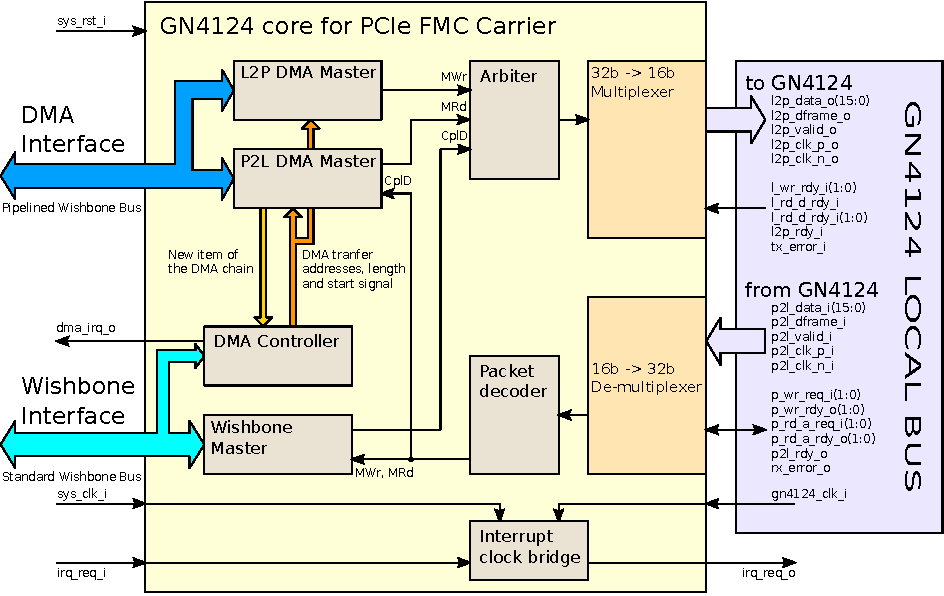
\includegraphics[width=0.9\textwidth]{GN4124core_arch.pdf}
   \caption{GN4124 core for PCIe FMC carrier}
   \label{fig:GN4124core_arch}
  \end{figure}

  The structure of this cores and some signals names are based on the Gennum cores \emph{Lambo} and \emph{Lotus}.

  The VHDL guidelines\footnote{See \href{http://www.ohwr.org/attachments/27/VHDLcoding.pdf}{http://www.ohwr.org/attachments/27/VHDLcoding.pdf}.} describes the rules used for writing the HDL code and the signals naming conventions.


 \section{De-multiplexer}
 This block takes the double data rate 16-bit P2L (PCI Express to Local
 Bus direction) bus from the GN4124 device and converts it to a single
 data rate 32-bit bus for use inside the GN4124 core.


 \section{Multiplexer}
 It takes the internal single data rate 32-bit data and transmits it as
 double data rate 16-bit data on the L2P (Local Bus to PCI Express
 direction) bus.


 \section{Packet decoder}
 This block extracts header information, address, data, byte enables,
 and timing controls of the packets from the GN4124 chip. It provides
 signals like:

 \begin{packed_item}
  \item Type of packet (target read request, target write request, master read completion \dots)
  \item Begin of packet
  \item Address that will increment with data for data block transfer (e.g. DMA transfers)
  \item Data
  \item End of packet
 \end{packed_item}


 \section{CSR Wishbone master}
 The CSR Wishbone master implements a master for the CSR Wishbone
 bus. CSR stands for Control and Status Registers. The CSR Wishbone bus
 is foreseen to access control, status and configuration registers of
 the cores inside the FPGA.
 It transforms a PCIe write into a Wishbone write and a PCIe read into a
 Wishbone read. Only single word reads and writes are supported on the
 Wishbone interface.
 The Wishbone master is using an external clock that can be different
 from the GN4124 core clock.

 Figure~\ref{fig:GN4124core_wb_master} shows the block diagram of the
 CSR Wishbone master.

 \begin{figure}[!ht]
  \centering
  \includegraphics[width=0.9\textwidth]{GN4124core_wb_master.pdf}
  \caption{CSR Wishbone master}
  \label{fig:GN4124core_wb_master}
 \end{figure}

 The target memory reads and target memory writes packets type coming
 from the decoder are routed to the CSR Wishbone master.
 The target address, the data (for the write cycles) and the cycle type
 (read or write) are pushed to a FIFO. The FIFO is used for
 synchronisation between the GN4124 core clock domain and the CSR
 Wishbone clock domain.

 The memory r/w requests are queued up at full local bus speed into the FIFO
 then the requests are played out at the Wishbone bus speed.
 When the FIFO is almost full the \verb+p_wr_rdy_o+ signal is
 de-asserted to indicate to the GN4124 that no more requests can be accepted.

 In case of memory read request, the data read back from the wishbone
 bus are pushed to another FIFO, also for syncronisation between the two
 clock domains. Then a read completion packet containing the read data
 is generated and sent to the arbiter.


\section{DMA Engine}

\subsection{DMA controller}

\begin{table}[htbp]
  \centering
  \begin{tabularx}{\textwidth}{|l|c|l|c|X|}                                                   \hline
    \textbf{NAME}  & \textbf{OFFSET} & \textbf{MODE} & \textbf{RESET} & \textbf{DESCRIPTION}  \\ \hline \hline
    DMACTRLR       & 0x00 & R/W & 0x00000000 & DMA engine control                                       \\ \hline
    DMASTATR       & 0x04 & RO  & 0x00000000 & DMA engine status                                              \\ \hline
    DMACSTARTR     & 0x08 & R/W & 0x00000000 & DMA start address in the carrier                               \\ \hline
    DMAHSTARTLR    & 0x0C & R/W & 0x00000000 & DMA start address (low) in the PCIe host                       \\ \hline
    DMAHSTARTHR    & 0x10 & R/W & 0x00000000 & DMA start address (high) in the PCIe host                      \\ \hline
    DMALENR        & 0x14 & R/W & 0x00000000 & DMA read length in bytes                                       \\ \hline
    DMANEXTLR      & 0x18 & R/W & 0x00000000 & Pointer (low) to next item in list                             \\ \hline
    DMANEXTHR      & 0x1C & R/W & 0x00000000 & Pointer (high) to next item in list                            \\ \hline
    DMAATTRIBR     & 0x20 & R/W & 0x00000000 & DMA chain control                                              \\ \hline
  \end{tabularx}
  \caption{Register set for the DMA controller block}
  \label{tab:dma_control}
\end{table}

\begin{figure}[!ht]
  \centering
  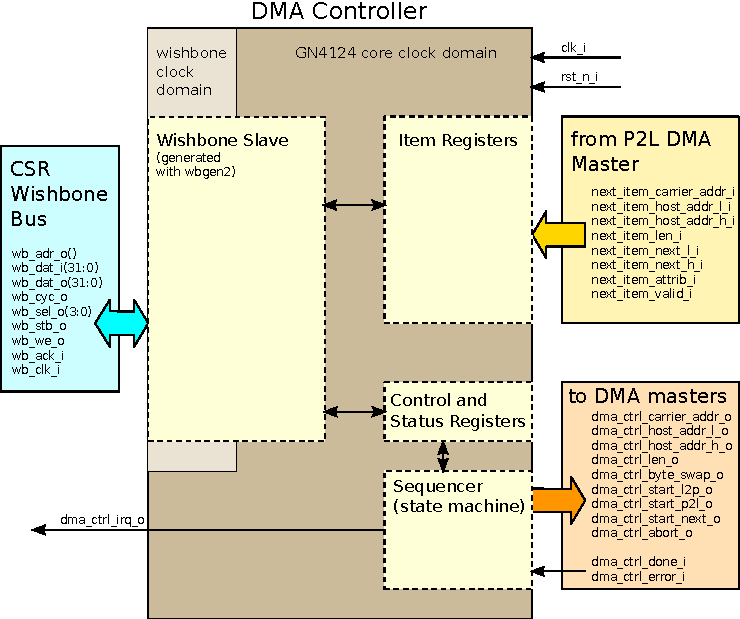
\includegraphics[width=0.9\textwidth]{GN4124core_DMA_controller.pdf}
  \caption{DMA controller}
  \label{fig:GN4124core_dma_ctrl}
\end{figure}

The DMA controller is a Wishbone slave controlled from the PCI Express host with the Wishbone master (see the functional specification). Figure \ref{fig:GN4124core_dma_ctrl} shows the internals of the DMA controller.

The transfer starts when the first bit (LSB) of the DMACTRLR (See table  \ref{tab:dma_control}) register is asserted. One of the two signals, \verb+dma_ctrl_start_L2P_o+ and \verb+dma_ctrl_start_P2L_o+, is set to '1' for one clock cycle. The \verb+dma_ctrl_start_L2P_o+ signal controls the DMA L2P master that performs transfers from the carrier to the PCI Express host and the \verb+dma_ctrl_start_P2L_o+ signal controls the DMA P2L master that performs transfers from the PCI Express host to the carrier.

The DMA controller waits for the \verb+dma_ctrl_done_i+ signal from one of the two DMA masters that indicates the end of the transfer. The \verb+dma_ctrl_error_i+ signal indicates the end of the current transfer if an error occurs.

After the end of a transfer, if this transfer is not the last, the controller ask to the P2L DMA master the new item of the DMA chain. The \verb+next_item_valid_i+ signal indicates that the DMA master can read the new DMA chain item from the P2L DMA master and starts the new cycle.

%\begin{figure}[!ht]
%  \centering
%    \includegraphics[width=0.8\textwidth]{State_Machine_DMA_controller_0.pdf}
%  \caption{DMA controller status}
%  \label{fig:GN4124core_dma_ctrl_status}
%\end{figure}

\begin{figure}[!ht]
 \centering
 %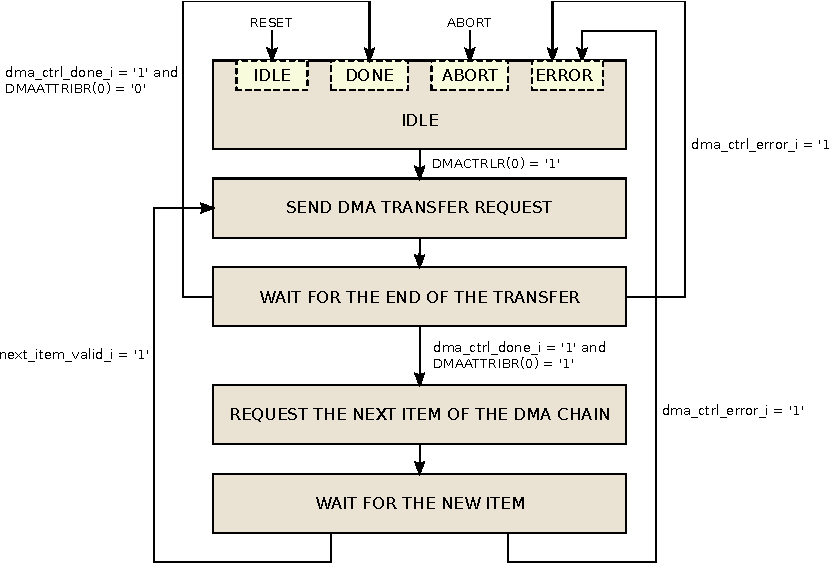
\includegraphics[width=0.8\textwidth]{State_Machine_DMA_controller.pdf}
 \includegraphics[width=0.8\textwidth]{dma_controller_state_machine.pdf}
 \caption{DMA controller state machine}
 \label{fig:GN4124core_dma_ctrl_state_machine}
\end{figure}

  \subsection{L2P DMA Master}
  The L2P DMA master (See figure \ref{fig:GN4124core_l2p_dma_master}) performs data transfers from the FMC carrier to the memory of the PCI Express host. The transfer is split in blocks of data with a maximal length of 4096 bytes. This is the maximal length of transfers allowed by the GN4124 chip.

  The L2P DMA master sends a master read request on the DMA interface and waits for answer. This transfer is clocked by the \verb+sys_clk_i+ signal. The received data are stocked in a FIFO that allows switching between clock domains.

  When the block of data is in the FIFO, the DMA master sends a master write request to the PCI Express host. This operation is clocked by the GN4124 Local Bus Clock. The transfer is paused if the \verb+l_wr_rdy_i+ signal from GN4124 chip is not asserted.



  \begin{figure}[!ht]
   \centering
   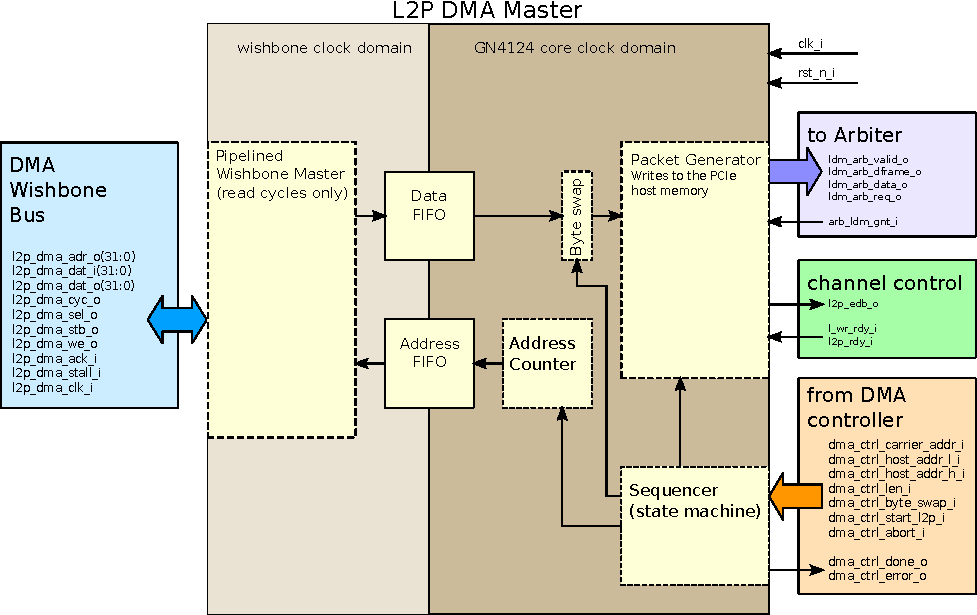
\includegraphics[width=0.9\textwidth]{GN4124core_L2P_DMA_master.pdf}
   \caption{L2P DMA master}
   \label{fig:GN4124core_l2p_dma_master}
  \end{figure}

  \subsection{P2L DMA Master}
  The P2L DMA master (See figure \ref{fig:GN4124core_p2l_dma_master}) performs data transfers from the PCI Express host to the FMC carrier. The transfer is split in blocks of data with a maximal length of 4096 bytes.

  The P2L DMA master sends a memory read request toward the GN4124 chip and waits for the answer. This operation is clocked by the GN4124 Local Bus Clock. The received data are stocked in a FIFO.

  When the block of data is in the FIFO, the DMA master starts a master write cycle on the DMA interface of this block. This transfer is clocked by the \verb+sys_clk_i+ signal.

  \begin{figure}[!ht]
   \centering
   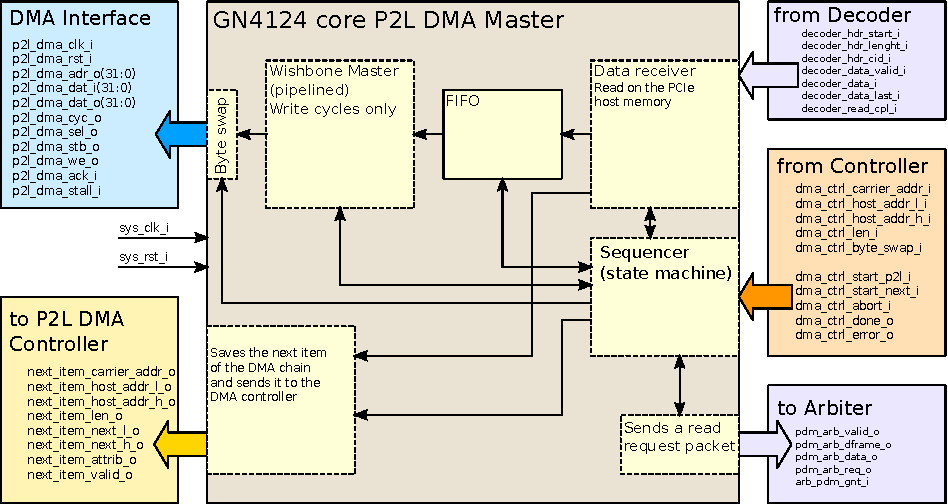
\includegraphics[width=0.9\textwidth]{GN4124core_P2L_DMA_master.pdf}
   \caption{P2L DMA master}
   \label{fig:GN4124core_p2l_dma_master}
  \end{figure}


 \section{Arbiter}
 Arbitrate between Wishbone master and the two DMA masters. The arbiter is waiting for a request signal from one of this blocks and it grants the bus to the first requester until the end of the packet.

 The highest priority is for the Wishbone master, then for the P2L DMA master, and the lower priority is for the L2P DMA master.


 \section{Interrupt clock bridge}
  It transforms input interrupt one-tick-long pulse clocked by \verb+sys_clk_i+ in a one-tick-long pulse clocked by the GN4124 local bus clock.
\end{document}

%
